\documentclass[a4paper, 14pt, dvipdfmx]{extarticle}

\usepackage{animate}
\usepackage{amsmath, amssymb, amsthm, mathrsfs, amsfonts, dsfont}
\usepackage{ascmac}
\usepackage{bbm}
\usepackage{bm}
\usepackage{breakcites}
\usepackage{calc}
\usepackage[style=base]{caption}
\usepackage{enumerate}
\usepackage[T1]{fontenc}
\usepackage{ifthen}
\usepackage{mathtools}
\usepackage{makecell}
\usepackage{mlmodern}
\usepackage{newtxtext}
\usepackage{optidef}
\usepackage[deluxe]{otf}
\usepackage{physics}
\usepackage{pifont}
\usepackage{setspace}
\usepackage{stfloats}
\usepackage{subcaption}
\usepackage{svg}
\usepackage{tikz}
\usepackage{xparse}
\usepackage[all]{xy}

\usepackage{float}
\usepackage{color}
\usepackage{graphicx}
\usepackage[margin=20truemm]{geometry}
\usepackage[colorlinks=true, allcolors=blue]{hyperref}

\usepackage{listings}

% === Commands ===

\definecolor{cA}{HTML}{0072BD}
\definecolor{cB}{HTML}{EDB120}
\definecolor{cC}{HTML}{77AC30}
\definecolor{cD}{HTML}{D95319}
\definecolor{cE}{HTML}{7E2F8E}
\newcommand{\cAText}[1]{\textcolor{cA}{#1}}
\newcommand{\cBText}[1]{\textcolor{cB}{#1}}
\newcommand{\cCText}[1]{\textcolor{cC}{#1}}
\newcommand{\cDText}[1]{\textcolor{cD}{#1}}
\newcommand{\cEText}[1]{\textcolor{cE}{#1}}
\newcommand{\red}[1]{\textcolor{red}{#1}}
\newcommand{\blue}[1]{\textcolor{blue}{#1}}
\newcommand{\green}[1]{\textcolor{green}{#1}}
\newcommand{\gray}[1]{\textcolor{gray}{#1}}
\newcommand{\black}[1]{\textcolor{black}{#1}}

\newcommand{\st}{\text{ s.t. }}
\newcommand{\Img}[1]{\mathrm{Im}\qty(#1)}
\newcommand{\Ker}[1]{\mathrm{Ker}\qty(#1)}
\newcommand{\Supp}[1]{\mathrm{supp}\qty(#1)}
\newcommand{\Rank}[1]{\mathrm{rank}\qty(#1)}
\newcommand{\floor}[1]{\left\lfloor #1 \right\rfloor}
\newcommand{\ceil}[1]{\left\lceil #1 \right\rceil}
% C++ (https://tex.stackexchange.com/questions/4302/prettiest-way-to-typeset-c-cplusplus)
\newcommand{\Cpp}{C\nolinebreak[4]\hspace{-.05em}\raisebox{.4ex}{\relsize{-3}{\textbf{++}}}}
% https://tex.stackexchange.com/questions/28836/typesetting-the-define-equals-symbol
\newcommand{\defeq}{\coloneqq}
\newcommand{\eqdef}{\eqqcolon}
% https://tex.stackexchange.com/questions/5502/how-to-get-a-mid-binary-relation-that-grows
\newcommand{\relmiddle}[1]{\mathrel{}\middle#1\mathrel{}}
\newcommand{\cmark}{\cCText{\ding{51}}} % check mark
\newcommand{\xmark}{\red{\ding{55}}} % cross mark

\DeclareMathOperator{\Proj}{Proj}
\DeclareMathOperator{\Exp}{Exp}
\DeclareMathOperator{\Hess}{Hess}
\DeclareMathOperator{\Retr}{Retr}
\DeclareMathOperator{\Span}{span}
\DeclareMathOperator{\myGrad}{grad}
\renewcommand{\grad}{\myGrad}

% https://tex.stackexchange.com/questions/564216/newcommand-for-each-letter
\ExplSyntaxOn
\NewDocumentCommand{\definealphabet}{mmmm}{
\int_step_inline:nnn{`#3}{`#4}{
\cs_new_protected:cpx{#1 \char_generate:nn{##1}{11}}{
\exp_not:N #2{\char_generate:nn{##1}{11}}}}}
\ExplSyntaxOff

\definealphabet{bb}{\mathbb}{A}{Z}
\definealphabet{rm}{\mathrm}{A}{Z}
\definealphabet{cal}{\mathcal}{A}{Z}
% \definealphabet{scr}{\mathscr}{A}{Z}
\definealphabet{frak}{\mathfrak}{a}{z}
\definealphabet{frak}{\mathfrak}{A}{Z}

% === Settings ===

% https://qiita.com/rityo_masu/items/efd44bc8f9229e014237
\allowdisplaybreaks[4]

\usetikzlibrary{
  3d,
  fit,
  calc,
  math,
  matrix,
  patterns,
  backgrounds,
  arrows.meta,
  decorations.pathmorphing,
}

\newcommand{\IMG}[2]{
    \begin{figure}[H]
        \centering
        \includegraphics[width={#2}\columnwidth]{#1}
    \end{figure}
}

\begin{document}

\title{Supplemental Material for 04/23\\Book Reading Seminar}
\author{Hiroki Hamaguchi}
\date{\today}
\maketitle

\begin{abstract}
    \begin{center}
        This is the supplemental material for the book reading seminar.

        Please refer to the textbook and the whiteboard for the main content.

        If necessary, please also refer to the \href{https://github.com/hari64boli64/BookReadingSeminarMaterials}{repository}.
    \end{center}
\end{abstract}

\section*{2.2}

\subsection*{2.2.1}

Lemma 1.19: For any $f \in C^2(\mathbb{R}^n)$,
and any $x, y \in \mathbb{R}^n$,
there exists $z \in [x, y]$ s.t.
\begin{equation*}
    f(y) = f(x) + \nabla f(x)^\top (y - x) + \frac{1}{2} (y - x)^\top \nabla^2 f(z) (y - x).
\end{equation*}

\begin{figure}[H]
    \centering
    \fbox{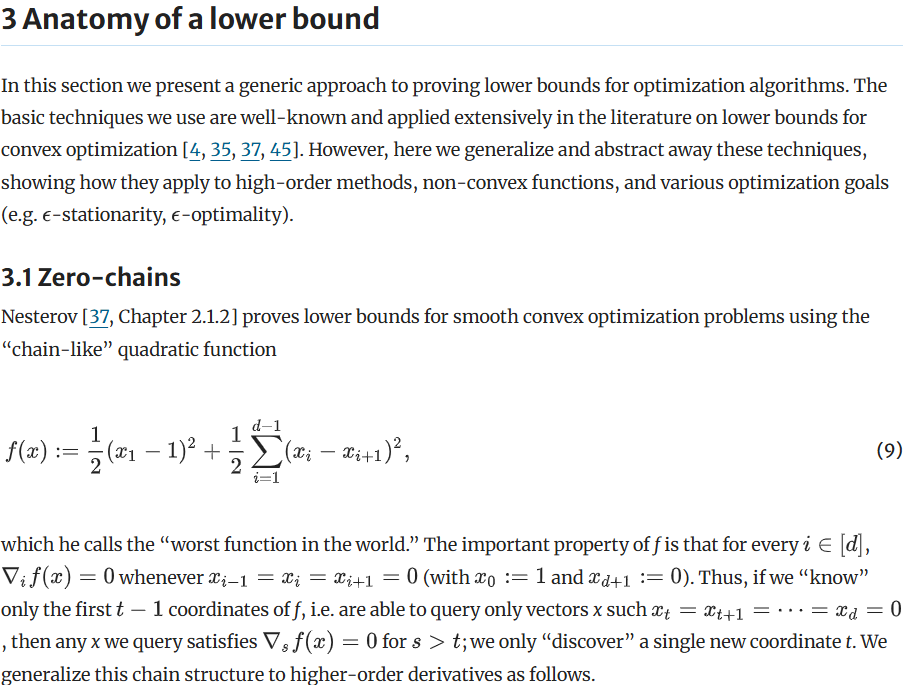
\includegraphics[width=0.7\columnwidth]{15.png}}
    \caption{[15]から引用}
\end{figure}

参考文献の[15]は、\href{https://link-springer-com.utokyo.idm.oclc.org/article/10.1007/s10107-019-01406-y}{Math. Program.}の2020年の論文。

\section*{2.3}

$A \succ O$ $\iff$ $\exists$ 直交行列 $Q$ と対角行列 $D$ s.t. $A=QDQ^\top$

\section*{2.4}

\subsection*{Ex.2.15}

一般に、
\begin{align*}
    f(y) & \geq f(x) + \langle \nabla f(x), y-x \rangle + \frac{\mu}{2}\norm{y-x}_2^2 \\
    f(x) & \geq f(y) + \langle \nabla f(y), x-y \rangle + \frac{\mu}{2}\norm{y-x}_2^2 \\
    0    & \geq \langle \nabla f(x)-\nabla f(y), y-x \rangle + \mu \norm{y-x}_2^2
\end{align*}
なので、
\begin{align*}
    \langle \nabla f(x)-\nabla f(y), x-y \rangle & \geq \mu \norm{y-x}_2^2   \\
    \langle \nabla f(x), x-x^* \rangle           & \geq \mu \norm{x-x^*}_2^2
\end{align*}
である。

Lemma 2.10より、
\begin{align*}
    \norm{x^{(k+1)}-x^*}_2^2 ={} & \norm{x^{(k)}-x^*}_2^2 - \frac1L\langle \nabla f(x^{(k)}), x^{(k)}-x^* \rangle + \frac{1}{L^2}\norm{\nabla f(x^{(k)})}_2^2 \\
    ={}                          & \norm{x^{(k)}-x^*}_2^2 - \frac1L\langle \nabla f(x^{(k)}), x^{(k)}-x^* \rangle                                             \\
                                 & -\frac1L\qty(\langle \nabla f(x^{(k)}), x^{(k)}-x^* \rangle - \frac{1}{L}\norm{\nabla f(x^{(k)})}_2^2)                     \\
    \leq{}                       & \norm{x^{(k)}-x^*}_2^2 - \frac{\mu}{L} \norm{x^{(k)}-x^*}_2^2
\end{align*}
途中でもLemma 2.10の証明中の式を使っている。

\subsection*{Ex.2.16}

特段の名前はついてない? 自信なし。

\subsection*{Ex.2.17}

\href{https://en.wikipedia.org/wiki/%C5%81ojasiewicz_inequality}{PL不等式}

\subsection*{Ex.2.18}

\begin{figure}[H]
    \centering
    \fbox{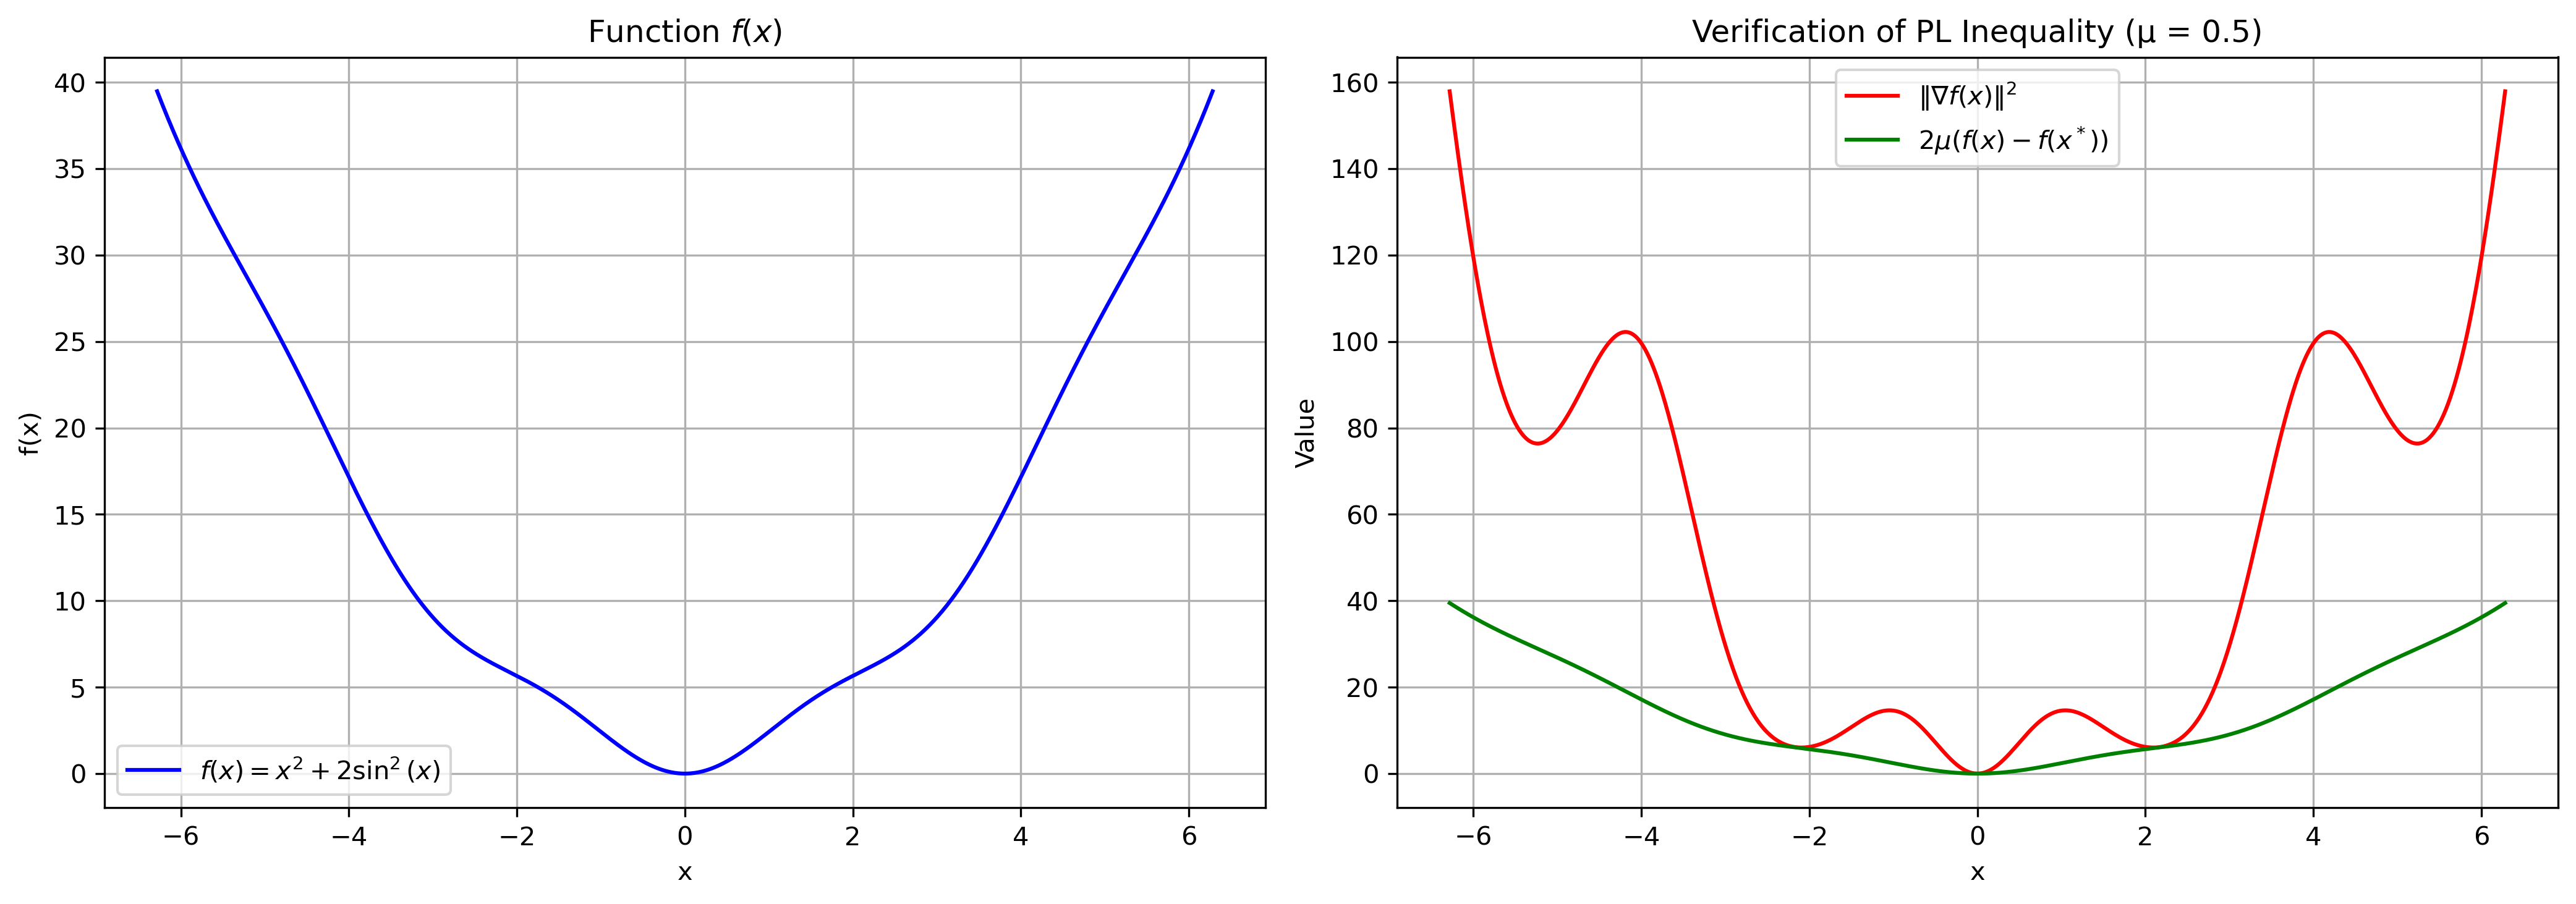
\includegraphics[width=0.95\columnwidth]{PL.png}}
    \caption{PL不等式を満たすが非凸な例}
\end{figure}

\section*{2.5}

\href{https://tm23forest.com/contents/linesearch-armijo-wolfe-condition-explained-visually}{直線探索}

\subsection*{Ex.2.20}

\begin{align*}
                                   & -c_1 h \norm{\nabla f(x)}_2^2                                                           \\
    \geq{}                         & f(x- h \nabla f(x)) - f(x)                                                              \\
    \geq{}                         & \nabla f(x)^\top ((x-h \nabla f(x)) - x) + \frac{\mu}{2} \norm{x-h \nabla f(x) - x}_2^2 \\
    ={}                            & -h \norm{\nabla f(x)}_2^2 + \frac{\mu}{2} h^2 \norm{\nabla f(x)}_2^2                    \\
    \therefore \quad -c_1 h \geq{} & -h + \frac{\mu}{2} h^2 \iff \frac{2(1-c)}{\mu} \geq h
\end{align*}

\begin{align*}
                          & c_2 \norm{\nabla f(x)}_2^2                                                \\
    \geq{}                & \nabla f(x)^\top \nabla f(x-h \nabla f(x))                                \\
    ={}                   & \nabla f(x)^\top (\nabla f(x) - \nabla^2 f(z) (h \nabla f(x)))            \\
    ={}                   & \norm{\nabla f(x)}_2^2 - h \nabla f(x)^\top \nabla^2 f(z) \nabla f(x)     \\
    \therefore c_2 \geq{} & 1 - h \lambda_{\max}(\nabla^2 f(z)) \geq 1-hL \iff h \leq \frac{1-c_2}{L}
\end{align*}

\href{https://m-katsurada.sakura.ne.jp/lecture/tahensuu1-2011/tahensuu1-2011-16/node2.html}{この証明はTaylor展開と積分の平均値の定理を経由して考えないと誤りかも}

\section*{2.6}

\subsection*{Ex.2.23}

不明。 私の頭が悪いだけかも知れません。

\noindent
$h(y/\alpha)$ と $y$ が $0$ を中心にスケーリングされているのが謎。
$x$ が中心では?

\subsection*{Projected Gradient Descent / Proximal Gradient Descent}

\href{https://qiita.com/hari64/items/f05fea3f9142826c1031}{参考}

\subsection*{Other assumptions}

\href{https://www.sciencedirect.com/science/article/pii/S1063520309000384}{参考文献[10] Iterative hard thresholding for compressed sensing}\\
\href{https://link-springer-com.utokyo.idm.oclc.org/article/10.1007/s00041-008-9035-z}{参考文献[10]の参考文献[1] Iterative Thresholding for Sparse Approximations}

\begin{figure}[H]
    \centering
    \fbox{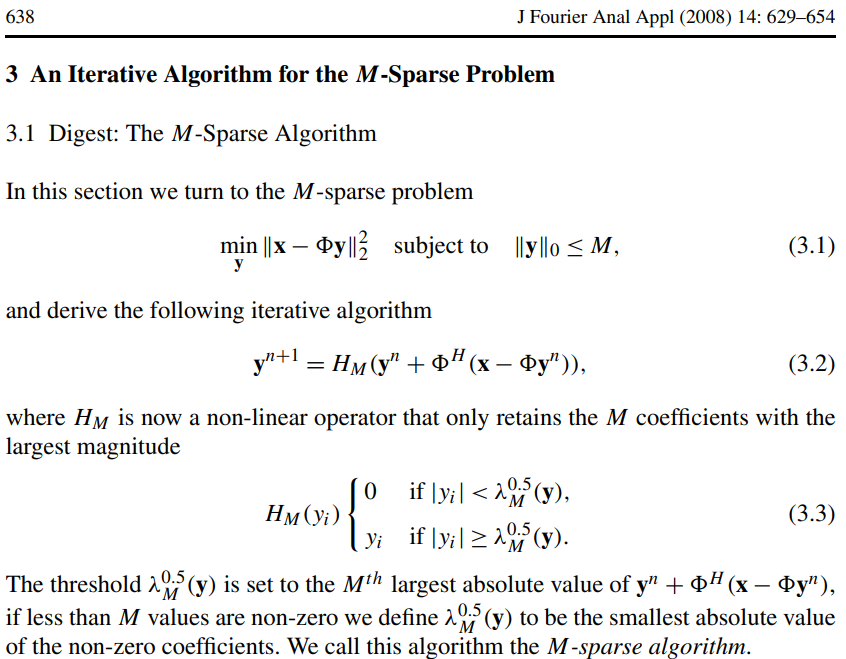
\includegraphics[width=0.8\columnwidth]{IHT.png}}
    \caption{Iterative Hard Thresholding}
\end{figure}

\section*{3}

もしここまで到達してしまったらすいません、お詫びします。
準備不足です。
質問とか大事な部分の深掘りとかで時間を使います。

\appendix

\section*{Appendix}

\lstinputlisting[caption=PL,label=code:PL,language=Python]{PL.py}

\end{document}
